% Authoritative RouterBSI_Draft_Appendix.docx; zero-based direct body paragraph IDs.

% DOCX-P002-BEGIN
\section{Introduction}
% DOCX-P002-END

% DOCX-P003-BEGIN
Large language model (LLM) agents increasingly rely on reusable skills to extend their capabilities beyond knowledge encoded in model parameters. These skills package procedural knowledge that can be reused across recurring classes of tasks. As skill libraries grow, however, explicitly exposing every available skill in the context becomes increasingly impractical. Recent work therefore shifts toward Skill Retrieval Augmentation (SRA), where skills must be retrieved and loaded from a large-scale skill corpora \citep{su2026skillretrieval} (Figure~\ref{fig:predicate-routing}).
% DOCX-P003-END

% INTEGRATION-BEGIN
\begin{figure}[!t]
\centering
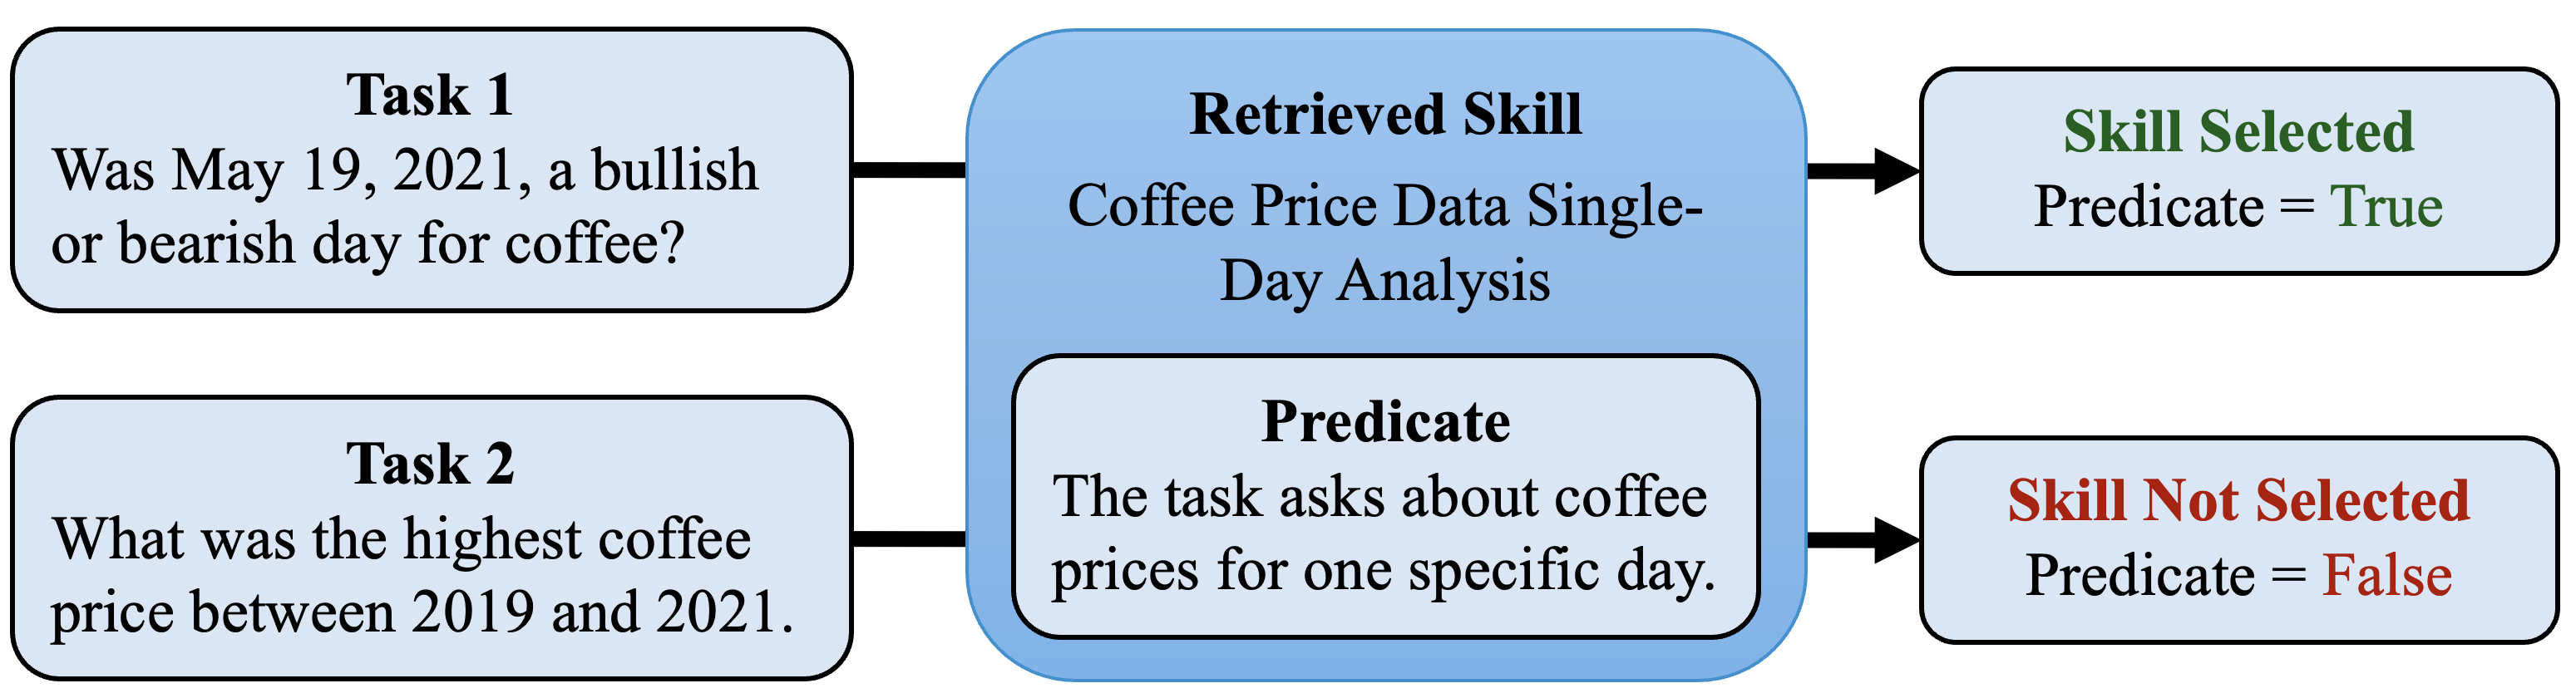
\includegraphics[width=\columnwidth]{figs/routing_figure.png}
\caption{Skill routing with a task applicability predicate. The skill is appropriately selected for task $q_{1}$ because the task asks about the price for a specific trading day. The skill is not accepted for task $q_{2}$ because it asks for the price between a range of years.}
\label{fig:predicate-routing}
\end{figure}
% INTEGRATION-END

% DOCX-P004-BEGIN
In SRA, retrieval based on semantic relevance alone is not enough. Skills must be invoked based on their downstream utility for completing a task to reliably augment the agent's capabilities. Current agents can struggle to distinguish useful skills from irrelevant ones even when the correct skill has been successfully retrieved \citep{su2026skillretrieval}. We refer to skill routing as the process of determining which retrieved candidate skills are applicable to a task and should therefore enter the agent\textquotesingle s active context for completing a task. Reliable routing must distinguish applicability from semantic relatedness: a skill can be topically similar to a task without satisfying the requirements under which its procedure should be invoked. This distinction becomes increasingly important as broader candidate sets introduce irrelevant procedures that can distract the model or interfere with downstream reasoning.
% DOCX-P004-END

% DOCX-P005-BEGIN
Existing routing approaches address this problem through similarity scores, learned utility functions, direct model-based selection, and explicit activation conditions. Learned retrievers and rerankers can improve discrimination among candidates but encode routing criteria implicitly in model parameters and require additional optimization data and compute. In contrast, non-parametric approaches keep the underlying model fixed while modifying external state that influences future decisions. Yet persistent external updates introduce a different reliability problem. An edit motivated by a failure can correct similar failure cases while undoing corrections to previously handled tasks or degrading performance on other cases. As interaction histories grow, retaining all prior examples for checking each update also makes continual adaptation increasingly expensive. This creates a need for a routing mechanism whose applicability criteria are explicit and editable, but whose updates are efficiencly constrained by prior experience and independently checked for generalization. These problems of controlling regressions while bounding used experience serve as the motivation for our approach.
% DOCX-P005-END

% DOCX-P006-BEGIN
We introduce RouterBSI, a recursive self-improving algorithm for skill routing in a black-box setting called RouterBSI. It refines task applicability predicates using Minimum Bayes Risk (MBR) with bounded replay to minimize errors on seen tasks and a held-out validation gate to reduce regressions on unseen tasks. The router evaluates predicates for top-k retrieved skills then selects skills if the task satisfies their respective predicate. RouterBSI improves its cold-start top-5 recall of required skills by an average of 24.9\% across different retrievers on tasks from TheoremQA, LogicBench, ToolQA, MedCalc-Bench, CHAMP, and BigCodeBench sharing a 26k skill corpus. On average, it retains 90.5\% of the required skills in top 5 from the top 50 skills retrieved. Its top-5 recall is 75.5\%, with relative recall improvements over baselines averaging 7.9\% to 33.6\% across retrievers.
% DOCX-P006-END

% DOCX-P007-BEGIN
Our contributions are:
% DOCX-P007-END

\begin{itemize}
\setlength{\itemsep}{0pt}
\setlength{\parsep}{0pt}

% DOCX-P008-BEGIN
\item 
We propose RouterBSI, a non-parametric skill-routing framework that evaluates explicit applicability predicates over retrieved candidates, making routing criteria interpretable and directly editable without updating the underlying language model.
% DOCX-P008-END

% DOCX-P009-BEGIN
\item 
We develop a recursive self-improvement procedure that refines predicates from routing failures, selects updates through minimum Bayes risk over a bounded replay of relevant and irrelevant tasks, and rejects updates with higher held-out validation error than the cold-start predicate.
% DOCX-P009-END

% DOCX-P010-BEGIN
\item 
We evaluate RouterBSI on six SRA-Bench datasets with a shared 26K-skill corpus, achieving the highest aggregate nDCG@10 and Hit@1 among evaluated methods while ablations establish the contributions of replay and validation.
% DOCX-P010-END

\end{itemize}
